\chapter*{付録A Raspberry Pi Cat}

\section{Raspberry Pi Cat}
Raspberry Pi Catは図\ref{fig:raspicat}で示された二輪の差動駆動型ロボットである.
このロボットについて説明をする.
\begin{figure}[H]
	\begin{center}
		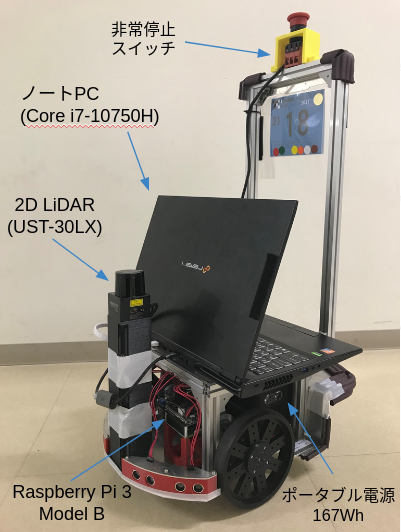
\includegraphics[width=0.5\linewidth]{figs/raspicat.png}
		\caption{}
		\label{fig:raspicat}
	\end{center}
\end{figure}

\subsection{ハードウェア構成}
\begin{figure}[H]
	\begin{center}
		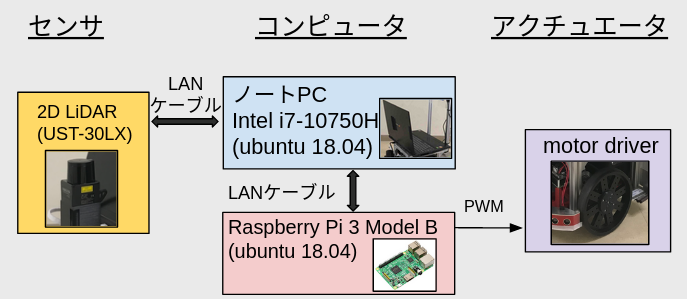
\includegraphics[width=1.0\linewidth]{figs/raspicat-hardware-config.png}
		\caption{}
		\label{fig:raspicat-hardware-config}
	\end{center}
\end{figure}

\subsection{ソフトウェア構成}

\begin{figure}[H]
	\begin{center}
		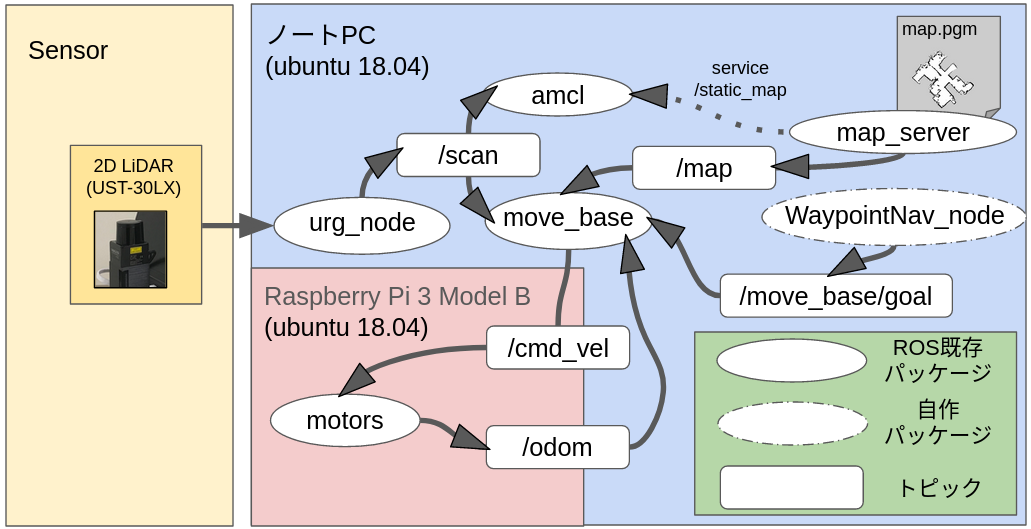
\includegraphics[width=1.0\linewidth]{figs/raspicat-software-config.png}
		\caption{}
		\label{fig:raspicat-software-config}
	\end{center}
\end{figure}

\subsection{使用したコンピュータのスペック}

\subsubsection{Raspberry Pi 3 Model B}
SoCはBroadcom BCM2837 1.2GHz×4(CPU).
メモリは1GB.
\subsubsection{ノートPC}
CPUはCore i7-10750H 2.6GHz×12. 
GPUはNVIDIA GeForce RTX 2070.
メモリは32GB.

\subsection{2D LiDAR}
使用した2D LiDARはHOKUYOのUST-30LXである.
UST-30LXの走査角度は270度, 角度分解能は0.25度, 測定分解能は1mm, 最大検出距離は60mである.

地面などのノイズを観測せずに多くのランドマークを獲得するために図\ref{fig:raspicat-lidar}
のように地面から36cmの高さに取り付けた.

\begin{figure}[H]
	\begin{center}
		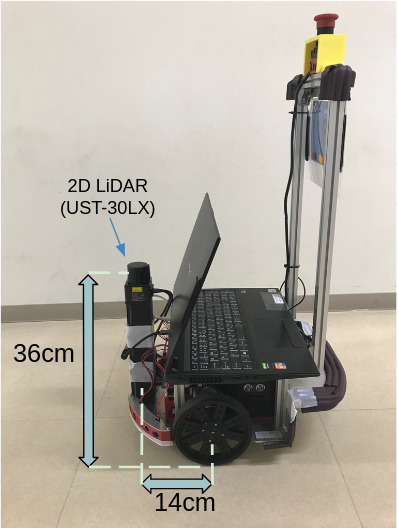
\includegraphics[width=0.5\linewidth]{figs/raspicat-lidar.png}
		\caption{}
		\label{fig:raspicat-lidar}
	\end{center}
\end{figure}

\subsection{アルミフレームによる高さ増し}
つくばチャレンジでのロボットの仕様条件を満たすために
図\ref{fig:raspicat-alumiframe}のようにアルミフレームを追加し, 高さ増しを行った.
元々のRaspberry Pi Catの高さは21cmであったが高さ増しを行うことによって
73cmになった。

\begin{figure}[H]
	\begin{center}
		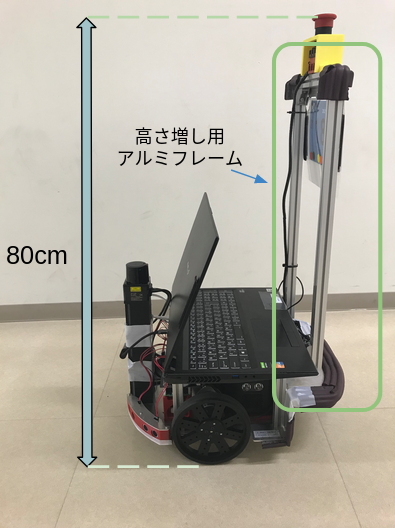
\includegraphics[width=0.5\linewidth]{figs/raspicat-alumiframe.png}
		\caption{}
		\label{fig:raspicat-alumiframe}
	\end{center}
\end{figure}